
\chapter{Changes in 0.7.2}
\label{ch:072changes}
The following update version complements the releases of PharmML 0.7 \& 0.7.1 
by few extensions or changes which will make the format more consistent 
and flexible. 



\section{Extensions/changes in ProbOnto}
\begin{itemize}
\item 
few new distributions have been added, see table \ref{figTable:univariates}, 
for example additional parameterisations of generalised Poisson, negative 
binomial and log-normal distributions.
\item 
Negative binomial -- changes in formulation/parameterisation for the NB1
have been introduced to account for the most common form. 
See a detailed discussion in appendix \ref{app:sec:NB1discussion}
\item 
more then 50 properties added, such as: linear combination, convolution, 
scaling, product, inverse, minimum, maximum, forgetfullness, residual, 
variate generation. See the excellent Leemis paper, \cite{Leemis:2008tg}, 
for definitions of these properties.
\item 
about 30 relationships between various distributions, most of them as 
described in Leemis, \cite{Leemis:2008tg}, see figure \ref{fig:POdiagram}.
\item 
about 35 reparameterisations between the members of normal, log-normal, 
negative binomial and generalised Poisson distributions families. Also indicated
in the figure \ref{fig:POdiagram}.
\end{itemize}


\begin{figure}[htb!]
\centering
\begin{tabular}{cc}
 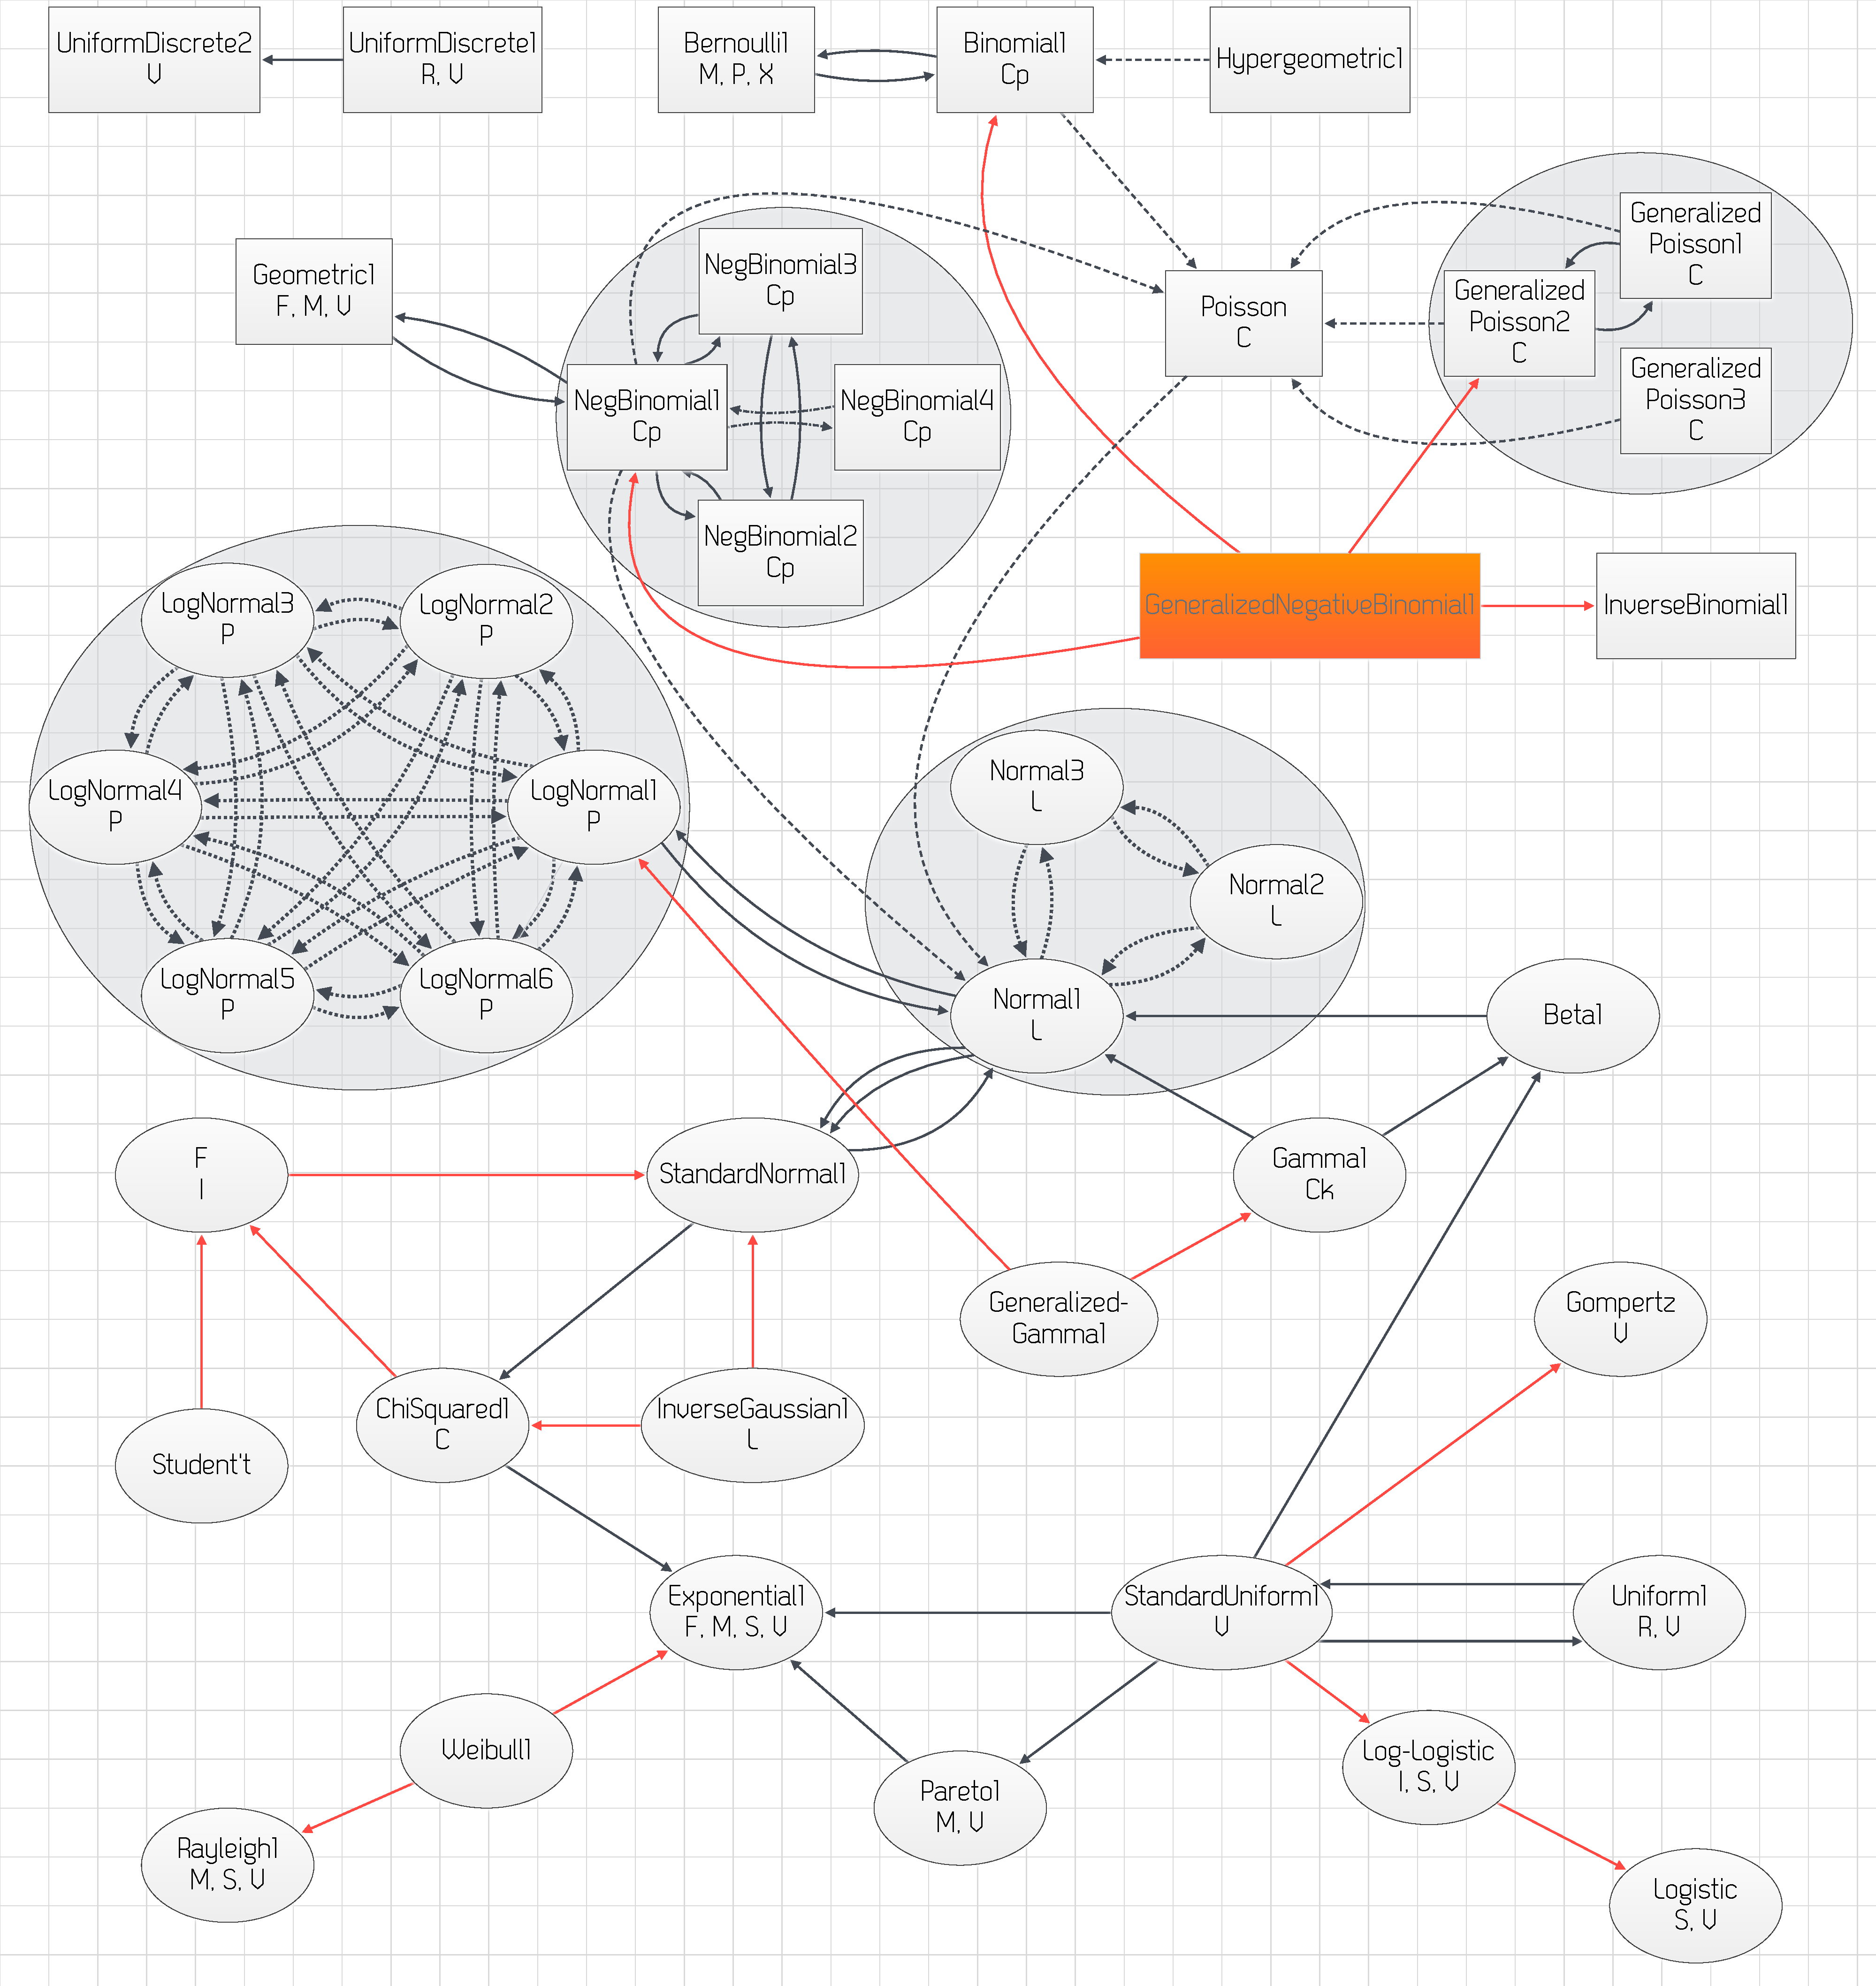
\includegraphics[width=140mm]{pics/POdiagram}
\end{tabular}
\caption{ProbOnto relationships diagram.}
\label{fig:POdiagram}
\end{figure}


\subsection{Changes and bug fixes in ProbOnto}
\begin{itemize}
\item 
Binomial distribution -- \xatt{numberOfTrials} instead of \xatt{numberOfFailures}
\end{itemize}


\section{New design tasks}

<ModellingSteps xmlns="http://www.pharmml.org/pharmml/0.7/ModellingSteps">

Target Tool with Target Tool Name

OptimalDesignStep

\begin{itemize}
\item 
Target tool reference
\item
OptimiseOn
\begin{itemize}
\item 
ArmSize
\item 
DoseAmount
\item 
DosingTimes
\item 
Duration
\item 
NumberArms
\item 
NumberSamples
\item 
NumberTimes
\item 
ObservationTimes
\item 
SymbRef
\end{itemize}
\item
FIM
\begin{itemize}
\item 
Matrix
\item 
File
\end{itemize}
\item 
Method
\begin{itemize}
\item 
Criterion: D, ED, ..., A
\item 
FIMfunction
\begin{itemize}
\item 
build-in types: trInv, det, ...
\item 
arbitrary expression
\end{itemize}
\item 
    ComputeFIM: FO. FOCE, ..., MCMC
\item 
    ApproximateFIM: full, ..., reducedParameterised
\item 
    TypeFIM: individual, population, Bayesian 
\item 
    DesignType: exact, statistical
\item 
    Optimization Algorithm: simplex, fw
\end{itemize}
\item 
Cost
\begin{itemize}
\item 
TotalCost
\item 
CostFunction
\begin{itemize}
\item 
build-in type: sample, individual
\item 
arbitrary expression
\end{itemize}
\end{itemize}
\item 
PriorInformation
\begin{itemize}
\item 
Matrix
\item 
File
\end{itemize}
\item 
Compute
\begin{itemize}
\item 
GraphOnly
\item 
PowerComparison
\item 
NSubjectComparison
\item 
PowerEquivalence
\item 
NSubjectEquivalence
\item 
EquivalenceRange
\item 
TypeIError
\item 
TypeIIError
\end{itemize}
\item 
SoftwareSettings
\begin{itemize}
\item 
File
\end{itemize}
\item 
Operation: evaluation OR optimisation
\begin{itemize}
\item 
Property, e.g. RtolEq, AtolEq, graph.logical, log.logical, graph.only, y.range
\end{itemize}
\end{itemize}


%</OptimalDesignStep>

\subsection{Implementation of evaluation and optimisation tasks}

The following listing exemplifies the available options in specifying an optimal 
design task. Covered are both sub-types
\begin{itemize}
\item 
evaluation
\item
optimisation
\end{itemize}
tasks. The \xelem{OptimalDesignStep} element contains all relevant elements. 
Note, the  that the information about the task's sub-type is stored within the 
\xelem{Operation} element which allows reuse existing structure and stay consistent
with previously supported \emph{Simulation} and \emph{Estimation} tasks.

\lstset{language=XML}
\begin{lstlisting}

    <ModellingSteps xmlns="http://www.pharmml.org/pharmml/0.7/ModellingSteps">
        
        <TargetTool oid="tTool">
            <TargetToolName>PFIM</TargetToolName>
        </TargetTool>
        
        <OptimalDesignStep oid="evaTask1">
            
            <TargetToolReference>
                <ct:OidRef oidRef="tTool"/>
            </TargetToolReference>
            
            <OptimiseOn>
                <ArmSize/>
                <DoseAmount>
                    <ct:Assign>
                        <ct:Real>100</ct:Real>
                    </ct:Assign>
                </DoseAmount>
                <DosingTimes/>
                <Duration/>
                <NumberArms/>
                <NumberSamples>
                    <ct:Assign>
                        <ct:Real>20</ct:Real>
                    </ct:Assign>
                </NumberSamples>
                <NumberTimes/>
                <ObservationTimes/>
                <ct:SymbRef symbIdRef="tdoseB"/>
                <ct:SymbRef symbIdRef="SEX"/>
            </OptimiseOn>
            
            <FIM symbId="FIM1">
                <ct:Matrix matrixType="Any">
                    <ct:MatrixRow>
                        <ct:Real>1.1</ct:Real>
                        <!-- omitted elements -->
                        <ct:Real>1.6</ct:Real>
                    </ct:MatrixRow>
                        <!-- omitted rows -->
                    <ct:MatrixRow>
                        <ct:Real>10.1</ct:Real>
                        <!--omitted elements-->
                        <ct:Real>10.6</ct:Real>
                    </ct:MatrixRow>
                </ct:Matrix>
                <!-- ALTERNATIVE to Matrix: FIM stored in an external 
                    file -->
                <!-- <File oid="FIMfile">
                    <ds:path>myFIM.csv</ds:path>
                </File>-->
            </FIM>
            <Method>
                <Criterion type="A"/>
                <FIMfunction type="trInv">
                    <ct:Assign>
                        <math:MatrixUniop op="trace">
                            <math:MatrixUniop op="inverse">
                                <ct:SymbRef symbIdRef="FIM1"/>
                            </math:MatrixUniop>
                        </math:MatrixUniop>
                    </ct:Assign>
                </FIMfunction>
                <!--ALTERNATIVE for FIMfunction: 
                    using build-in operator types, here 'trInv' 
                    which is identical to the explicit expression 
                    above-->
                <!-- <FIMfunction type="trInv">     
                    <ct:Assign>
                        <ct:SymbRef symbIdRef="FIM1"/>
                    </ct:Assign>
                </FIMfunction>-->
                <ComputeFIM type="FO"/>
                <ApproximateFIM type="full"/>
                <TypeFIM type="population"/>
                <DesignType type="exact"/>
                <OptimizationAlgorithm type="FedorovWynn"/>
            </Method>
            <Cost>
                <TotalCost>
                    <ct:Assign>
                        <ct:Real>1.3</ct:Real>
                    </ct:Assign>
                </TotalCost>
                <CostFunction type="sample"/>
            </Cost>
            <PriorInformation>
                <ct:Matrix matrixType="Any">
                    <ct:MatrixRow>
                        <ct:Real>1.1</ct:Real><!-- omitted elements --><ct:Real>1.6</ct:Real>
                        <!-- omotted rows -->
                        <ct:Real>10.1</ct:Real><!-- omitted elements --><ct:Real>10.6</ct:Real>
                    </ct:MatrixRow>
                </ct:Matrix>
                <!-- ALTERNATIVE to Matrix: prior information matrix stored 
                    in an external file -->
                <!-- <File oid="priorIMfile">
                    <ds:path>myPriorIM.csv</ds:path>
                </File>-->
            </PriorInformation>
            <Compute>
                <GraphOnly>
                    <ct:Assign>
                        <ct:False/>
                    </ct:Assign>
                </GraphOnly>
                <PowerComparison>
                    <ct:Assign>
                        <ct:True/>
                    </ct:Assign>
                </PowerComparison>
                <NSubjectComparison>
                    <ct:Assign>
                        <ct:True/>
                    </ct:Assign>
                </NSubjectComparison>
                <PowerEquivalence>
                    <ct:Assign>
                        <ct:Real>0.8</ct:Real>
                    </ct:Assign>
                </PowerEquivalence>
                <NSubjectEquivalence>
                    <ct:Assign>
                        <ct:True/>
                    </ct:Assign>
                </NSubjectEquivalence>
                <EquivalenceRange>
                    <ct:Assign>
                        <ct:Interval>
                            <ct:LeftEndpoint>
                                <ct:Assign>
                                    <math:Uniop op="log">
                                        <ct:Real>0.8</ct:Real>
                                    </math:Uniop>
                                </ct:Assign>
                            </ct:LeftEndpoint>
                            <ct:RightEndpoint>
                                <ct:Assign>
                                    <math:Uniop op="log">
                                        <ct:Real>1.2</ct:Real>
                                    </math:Uniop>
                                </ct:Assign>
                            </ct:RightEndpoint>
                        </ct:Interval>
                    </ct:Assign>
                </EquivalenceRange>
                <TypeIError>
                    <ct:Assign>
                        <ct:Real>0.05</ct:Real>
                    </ct:Assign>
                </TypeIError>
                <TypeIIError>
                    <ct:Assign>
                        <ct:Real>0.9</ct:Real>
                    </ct:Assign>
                </TypeIIError>
            </Compute>
            <SoftwareSettings>
                <File oid="softSettingsOID">
                    <ds:path>mySettings.xml</ds:path>
                </File>
            </SoftwareSettings>
            
            <Operation opType="evaluation" order="1">
                <Property name="RtolEq">
                    <ct:Assign>
                        <ct:Real>1E-06</ct:Real>
                    </ct:Assign>
                </Property>
                <Property name="AtolEq">
                    <ct:Assign>
                        <ct:Real>1E-06</ct:Real>
                    </ct:Assign>
                </Property>
                <Property name="graph.logical">
                    <ct:Assign>
                        <ct:True/>
                    </ct:Assign>
                </Property>
                <Property name="log.logical">
                    <ct:Assign>
                        <ct:String>'y'</ct:String>
                    </ct:Assign>
                </Property>
                <Property name="graph.onf">
                    <ct:Assign>
                        <ct:Real>0</ct:Real>
                    </ct:Assign>
                </Property>
                <Property name="y.range">
                    <ct:Assign><ct:Interval>
                        <ct:LeftEndpoint>
                            <ct:Assign>
                                <ct:Real>0</ct:Real>
                            </ct:Assign>
                        </ct:LeftEndpoint>
                        <ct:RightEndpoint>
                            <ct:Assign>
                                <ct:Real>10</ct:Real>
                            </ct:Assign>
                        </ct:RightEndpoint>
                    </ct:Interval></ct:Assign>
                </Property>
            </Operation>
        </OptimalDesignStep>
\end{lstlisting}



\section{Time-to-Event modeling}

Hazard/survival function added to mode common models
\begin{itemize}
\item 
Weibull
\item 
Exponential
\item 
Rayleigh
\item 
Gompertz 
\item 
Lognormal
\end{itemize}


\section{Removing redundant elements}
Removing parameter elements -- not used and not required
IntensityParameter

        
\section{Minor changes}
\begin{itemize}
\item 
Vector can be empty with elements defend using the \xatt{default}
attribute, similarly to what is possible when defining matrices. With this
feature a \emph{null} vector, one whose all elements are zero.
\item
new \xatt{determinant} matrix operator has been defined.
\end{itemize}













